% Physics experiment report
% 20/Oct/2016

\documentclass[a4paper,10pt,notitlepage]{report}

\usepackage{CJKutf8}
\usepackage{amsmath}
\usepackage{indentfirst}
\usepackage{graphicx}

\setlength{\parindent}{2em} 

\begin{CJK*}{UTF8}{gbsn}
\begin{document}

\title{测量误差和数据处理实验报告}
\author{秦光辉\ 9组3号}
\maketitle

\section*{一,实验数据处理}

	表一是实验数据.D是钢杯外径,d是钢杯内径,H是外部杯高,h是内部杯高.游标卡尺的允差为e=0.002cm. \\
	
\begin{table}[htbp]
\centering
	\begin{tabular}{|c|c|c|c|c|}
	
		\multicolumn{5}{c}{Table 1\ 游标卡尺测钢杯含钢体积} \\
		\hline
		item & D/cm & d/cm & H/cm & h/cm \\
		\hline
		零点读数 & \multicolumn{4}{c}{-0.002} \vline \\
		\hline
		\# 1 & 2.803 & 1.980 & 4.468 & 3.264 \\
		\hline
		\# 2 & 2.806 & 1.984 & 4.466 & 3.260 \\
		\hline
		\# 3 & 2.806 & 1.982 & 4.472 & 3.256 \\
		\hline
		\# 4 & 2.802 & 1.976 & 4.466 & 3.262 \\
		\hline
		\# 5 & 2.807 & 1.978 & 4.470 & 3.256 \\
		\hline
		\# 6 & 2.804 & 1.980 & 4.472 & 3.258 \\
		\hline
		平均值 & 2.805 & 1.980 & 4.470 & 3.259 \\
		\hline
		标准差 & 0.001 & 0.002 & 0.002 & 0.002 \\
		\hline
		考虑仪器允差后的标准差 & 0.003 & 0.003 & 0.003 & 0.003\\
		\hline
		修正零点后的平均值 & 2.807 & 1.982 & 4.472 & 3.261\\
		\hline

	\end{tabular}
\end{table}

	测量结果为 \\
	
\begin{align}
	\bar{D} \pm \sigma_{D} &= 2.807 \pm 0.003 cm \\
	\bar{d} \pm \sigma_{d} &= 1.982 \pm 0.003 cm \\
	\bar{H} \pm \sigma_{H} &= 4.472 \pm 0.003 cm \\
	\bar{h} \pm \sigma_{h} &= 3.261 \pm 0.003 cm
\end{align}

	计算结果是 \\
	
\begin{align}
	\bar{V} &= \frac{\pi}{4}(\bar{D}^2 \bar{H} - \bar{d}^2 \bar{h}) = 17.613 cm^3 \\
	\sigma_V &= \frac{\pi}{4}\sqrt{(2DH \times \sigma_D)^2 + (D^2 \times \sigma_H)^2 + (2dh \times \sigma_d)^2 + (d^2 \times \sigma_h)^2} \\
	& = 0.06 cm^3 \\
	V &= 17.61 \pm 0.06 cm^3
\end{align}

	表二是是螺旋测微器测小钢球体积的实验数据.零点为$d_0$.螺旋测微计的允差为e=0.001cm. \\
	
\begin{table}[htbp]
\centering
	\begin{tabular}{|c|c|c|c|c|c|c|}
	
		\multicolumn{7}{c}{Table 2\ 螺旋测微器测小钢球体积实验数据} \\
		\multicolumn{7}{l}{\scriptsize{unit: cm}} \\
		\hline
		\# & 1 & 2 & 3 & 4 & 5 & 6 \\
		\hline
		$d_i$ & 1.2722 & 1.2719 & 1.2718 & 1.2718 & 1.2719 & 1.2721 \\
		\hline

	\end{tabular}
\end{table}
	
\begin{equation}
	d_0 = 0.0022cm
\end{equation}
	
	数据处理过程见式(10)到(17),$\bar{d'}$表示考虑零点偏差之前的读数,$\bar{d}$表示考虑零点偏差之后的读数,$\sigma_{\bar{d}}$是d平均值的标准差,$\sigma_d$是考虑仪器允差之后d的标准差,$\sigma_V$是V的标准差. \\
		
\begin{align}
	&\bar{d'} = 1.2720cm \\
	&\bar{d} = 1.2618cm \\
	&\sigma_{\bar{d}} = 0.0001cm \\
	&\sigma_d = 0.001cm \\
	&\bar{d} \pm \sigma_d = 1.262 \pm 0.001 cm \\
	&V = \frac{\pi \bar{d}^3}{6} = 1.0523 cm^3 \\
	&\sigma_V = \frac{pi}{6} \times 3d^2 * \sigma_d = 0.003cm^3 \\
	&V \pm \sigma_V = 1.052 \pm 0.003 cm^3
\end{align}
	
\section*{二,习题}
\subsection*{1}
	
	(1)0.0001cm 一位 \\
	
	(2)1.000s 四位 \\
	
	(3)2.7 $\times$ $10^{20}$ J 二位 \\
	
	(4)980.120 $\times cm \cdot s^{-2}$ 六位 \\

\subsection*{2}

	(1)

\begin{align}
	&\frac{1}{\frac{1}{a} - \frac{1}{b}} cm = \frac{1}{0.10 \underline{10} - 0.001000 \underline{10}} cm = \frac{1}{0.10\underline{00}} cm = 10.0 cm  \\
	&c \pm e_c = 10.0 \pm 0.1
\end{align}

	(2)

	x的极限误差 \\
	
\begin{equation}
	e_x = 0.01
\end{equation}

	且有

\begin{align}
	&e_x \times \frac{dy}{dx} | _{x = 9.24} = -1.5 \times 10^{-38} \\
	&y = 8 \times 10^{-38} \\
	&y \pm e_y = ( 8 \pm 2) \times 10^{-38}
\end{align}
	
	(3)

\begin{align}
	&e_x = 0.1 \\
	&\frac{dy}{dx} | _{x = 56.7} = 0.0176 \\
	&e_y = e_x * 0.0176 = 0.00176 \\
	&y = 4.038 \\
	&y \pm e_y = 4.038 \pm 0.002
\end{align}

	(4)
	
\begin{align}
	&e_x = 1' \\
	&e_y = \frac{dy}{dx} | _{x = 56.7} \times 1' = -4.75 \times 10^{-5} \\
	&y = 0.98657 \\
	&y \pm e_y = 9.8657 \pm 0.0005 \times 10^{-1}
\end{align}

\subsection*{3}

	(1)

\begin{align}
	&\frac{\partial \rho}{\partial m_1} = - \frac{\rho_0 m_2}{(m_1 - m_2)^2} \\
	&\frac{\partial \rho}{\partial m_2} = \frac{\rho_0 m_1}{(m_1 - m_2)^2} \\
	&\sigma_\rho = \sqrt{(\frac{\partial \rho}{\partial m_1} \times \sigma_{m_1})^2 + (\frac{\partial \rho}{\partial m_2} \times \sigma_{m_2})^2} \\
	&= \frac{\rho_0}{(m_1 - m_2)^2}\sqrt{(m_2 \sigma_{m_1})^2 + (m_1 \sigma_{m_2})^2}
\end{align}

	(2)
	
\begin{align}
	&\frac{\partial y}{\partial a} = \frac{b}{a(a+b)} \\
	&\frac{\partial y}{\partial b} = \frac{a}{b(a+b)} \\
	&\sigma_y = \sqrt{(\frac{\partial y}{\partial a} \times \sigma_a)^2 + (\frac{\partial y}{\partial b} \times \sigma_b)^2} \\
	& = \frac{1}{|a+b|}\sqrt{(\frac{b}{a}\sigma_a)^2 + (\frac{a}{b}\sigma_b)^2}
\end{align}

\subsection*{4}

	方法一:

\begin{align}
	&L = L_1 + \frac{d_1}{2} + \frac{d_2}{2} \\
	&\sigma_L = \sqrt{\sigma_{L_1}^2 + \frac{\sigma_{d_1}^2}{4} + \frac{\sigma_{d_2}^2}{4} } = 0.9 \mu m
\end{align}

	方法二:
	
\begin{align}
	&L = L_2 - \frac{d_1}{2} - \frac{d_2}{2} \\
	&\sigma_L = \sqrt{\sigma_{L_2}^2 + \frac{\sigma_{d_1}^2}{4} + \frac{\sigma_{d_2}^2}{4} } = 1 \mu m
\end{align}

	方法三:
	
\begin{align}
	&L = \frac{L_1 + L_2}{2} \\
	&\sigma_L = \sqrt{\frac{\sigma_{L_1}^2}{4} + \frac{\sigma_{L_2}^2}{4} } = 0.6 \mu m
\end{align}

	应当选择第三个方法.
	
\section*{5}

	因: \\
	
\begin{equation}
	S = L_1 L_2 - \frac{\pi}{4} d_1^2 - \frac{\pi}{4} d_2 ^ 2 \approx 63 cm^2	
\end{equation}

	故相对不确定度:

\begin{align}
	&\frac{\sigma_S}{S} = \frac{\sqrt{(L_2\sigma_{L_1})^2+(L_1\sigma_{L_2})^2+(\frac{\pi}{2}d_1\sigma_{d_1})^2+(\frac{\pi}{2}d_2\sigma_{d_2})^2}}{L_1 L_2 - \frac{\pi}{4} d_1^2 - \frac{\pi}{4} d_2 ^ 2} 	
\end{align}

	若要$\frac{\sigma_S}{S}\leq0.5\%$,代入数据知:

\begin{equation}
	\sigma_{d_2}\leq 1 cm
\end{equation}

	可见小孔的大小即使不测,最后面积的测量的误差也不会超过$0.5\%$.
	
\section*{7}

	(1)我们有公式
	
\begin{align}
	g = \frac{2h}{t^2}
\end{align}

	由于尺子和钟表有误差,我们有:

\begin{align}
	&h_0=h_1(1+\alpha \Delta T) \\
	&t_0=t_1(1+1\times 10^{-4})
\end{align}

	代入$\alpha=1\times 10{-5}$及$\Delta T=10$知:

\begin{align}
	g_1&=g_0(1+1\times 10^{-4}) \\
	&=980.1 cm/s^2 \\
	\Delta g&=g_1-g_0=1\times 10^{-4} g_0=0.1cm/s^2
\end{align}

	(2)单摆周期的准确度为: 
	
\begin{equation}
\frac{\Delta T}{T}=\frac{1}{4} sin^2(\frac{\theta}{2})
\end{equation}

	要求准确度$\leq 0.5\%$,则: 

\begin{align}
	&\frac{\Delta T}{T}=\frac{1}{4} sin^2(\frac{\theta}{2})\leq 0.5\%\\
	& \theta \leq 16^\circ
\end{align}

	要求准确度$\leq 0.05\%$,则:

\begin{align}
	&\frac{\Delta T}{T}=\frac{1}{4} sin^2(\frac{\theta}{2})\leq 0.05\%\\
	& \theta \leq 5^\circ
\end{align}

\section*{10}

	由最小二乘法得到:
	
\begin{align}
	\lambda&=\sum_{i=1}^n {\frac{(i-\bar{i})y_i}{\sum_{i=1}^n {(i-\bar{i})^2}}} =8.7528mm \\
	y &= (18.71 + 8.7528i) mm
\end{align}

	同时有:

\begin{align}
	&\sigma_y=\sqrt{\frac{e^2}{3}+\frac{e_{y_i}^2}{3}}=0.07mm\\
	&\sigma_{\lambda}=\frac{\sigma_y}{\sqrt{\sum_{i=1}^{10} {(i-\bar{i})^2}}}=0.0007mm
\end{align}

	$\lambda$的不确定度为:
	
\begin{equation}
	\lambda=8.7528\pm0.0007 mm
\end{equation}

	$f$的不确定度为:

\begin{equation}
	\sigma_f=\frac{0.05}{\sqrt{3}}=0.03 kHz
\end{equation}

	所以:

\begin{equation}
	f=39.58\pm0.03 kHz
\end{equation}

	可以得到这中实验条件下的声速测量值:

\begin{align}
	&c=f\lambda=346.4 m/s\\
	&\sigma_c=\sqrt{f^2\sigma_{\lambda}^2+\lambda^2\sigma_f^2}=0.3m/s\\
	&c=346.4\pm0.3 m/s
\end{align}

\section*{11}

	(1)见图一,从图中可以看出这是线性关系 \\
	
\begin{figure}
\centering
	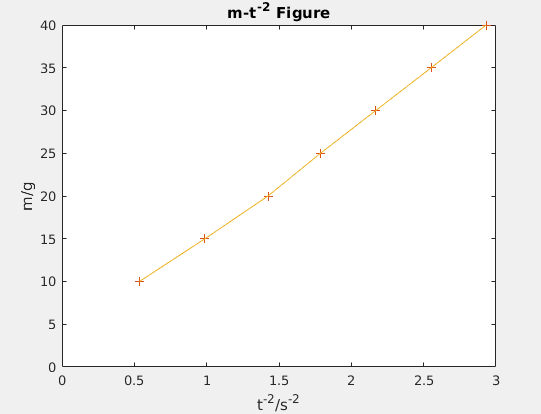
\includegraphics[scale=0.5]{Q11.png}
	\caption{图一\ m-$\frac{1}{t^2}$图线}
\end{figure}

	(2)	由表格中的数据可计算得:

\begin{align}
	&\overline{m} =25.00 \\
	&\overline{\frac{1}{t^2}} =1.770 \\
	&\overline{m^2}=725.00 \\
	&\overline{\frac{1}{t^2}^2} =3.757 \\
	&\overline{m\frac{1}{t^2}}=\overline{\frac{1}{t^2}m}=52.14 
\end{align}
	
	如果$m$为横坐标,$\frac{1}{t^2}$为纵坐标:

\begin{align}
	&k_2=\frac{\overline{m\frac{1}{t^2}}-\overline{m}\overline{\frac{1}{t^2}}}{\overline{m^2}-\overline{m}^2}=0.0790 \\
	&b_2=\overline{\frac{1}{t^2}}-k_2\overline{m}=-0.206 \\
	&r_2=\frac{\overline{m\frac{1}{t^2}}-\overline{m}\overline{\frac{1}{t^2}}}{\sqrt{(\overline{m^2}-\overline{m}^2)(\overline{\frac{1}{t^2}^2}-\overline{\frac{1}{t^2}}^2)}}=0.9993
\end{align}

	(3)如果$m$为纵坐标,$\frac{1}{t^2}$为横坐标:
	
\begin{align}
	&k_1=\frac{\overline{m\frac{1}{t^2}}-\overline{m}\overline{\frac{1}{t^2}}}{\overline{\frac{1}{t^2}^2}-\overline{\frac{1}{t^2}}^2}=12.64 \\
	&b_1=\overline{m}-k_2\overline{\frac{1}{t^2}}=2.64 \\
	&r_1=\frac{\overline{m\frac{1}{t^2}}-\overline{m}\overline{\frac{1}{t^2}}}{\sqrt{(\overline{m^2}-\overline{m}^2)(\overline{\frac{1}{t^2}^2}-\overline{\frac{1}{t^2}}^2)}}=0.9993
\end{align}

	(4)从计算结果和表达式都可以看出:
	
\begin{equation}
	r_1=r_2
\end{equation}

	从表达式可以直接得到

\begin{equation}
	r_1=r_2=\frac{\overline{m\frac{1}{t^2}}-\overline{m}\overline{\frac{1}{t^2}}}{\sqrt{(\overline{m^2}-\bar{m}^2)(\overline{\frac{1}{t^2}^2}-\bar{\frac{1}{t^2}}^2)}}=\sqrt{k_1k_2}
\end{equation}

\section*{三,分析与讨论}

\subsection*{1.结合实测数据分析系统误差和随机误差对于钢杯体积不确定度的贡献}

	在测量小钢杯的体积过程中,每个数据都测了6次.在这样多次的重复测量下,系统的随机误差依然没有降到很低,原因是有些物理量非常不好测.比如深度h,由于小钢杯内壁和底部之间并不垂直,很难保证游标卡尺和底部保持垂直.又由于工差等原因,钢杯上下底面并不平行,测量过程中难免产生很多误差.这些都制约着测量的精度. \\
	
	从数据来看,随机误差贡献的不确定度和仪器允差大致相等,仪器允差贡献略高于随机误差.例如在D的测量中,随机误差在0.001cm以下,而允差则是0.003cm. \\
	
\subsection*{2.结合实测数据分析系统误差和随机误差对于小钢球体积不确定度的贡献}

	在测量钢球体积过程中,一共测量了6次直径.小球做工比较好,各个角度的直径大致相等,在6次实验测量下随机误差非常小,在0.0001cm的量级,而系统允差却为0.001cm,可见在这次实验中,随机误差对实验造成的影响远小于系统允差. \\

\section*{四,感悟和收获}

	这个实验是一个非常基础的实验,真正的实验过程没有超过二十分钟,但是却非常有意义.物理实验中无法避免的会有很多误差,但是我们却可以使用各种统计学上的办法分析误差,确定不确定度范围,从而分析实验结果.如果没有不确定度分析,实验结果的好坏,实验结果对理论是验证还是推翻这些问题都无从探讨.虽然基础物理实验几乎不可能会有什么新的发现,但是这种严谨的科学态度确实值得需要从现在就开始培养! \\

\end{CJK*}
\end{document}
